\thispagestyle{quantoannone}
\pagestyle{quantoan}
\everymath{\color{quantoan}}
\graphicspath{{../quantoan/pic/}}
%\blfootnote{\color{quantoan}\color{quantoan}$^*$Nguồn Math. Intellegencer, Số $41$.}
\begingroup
\AddToShipoutPicture*{\put(0,616){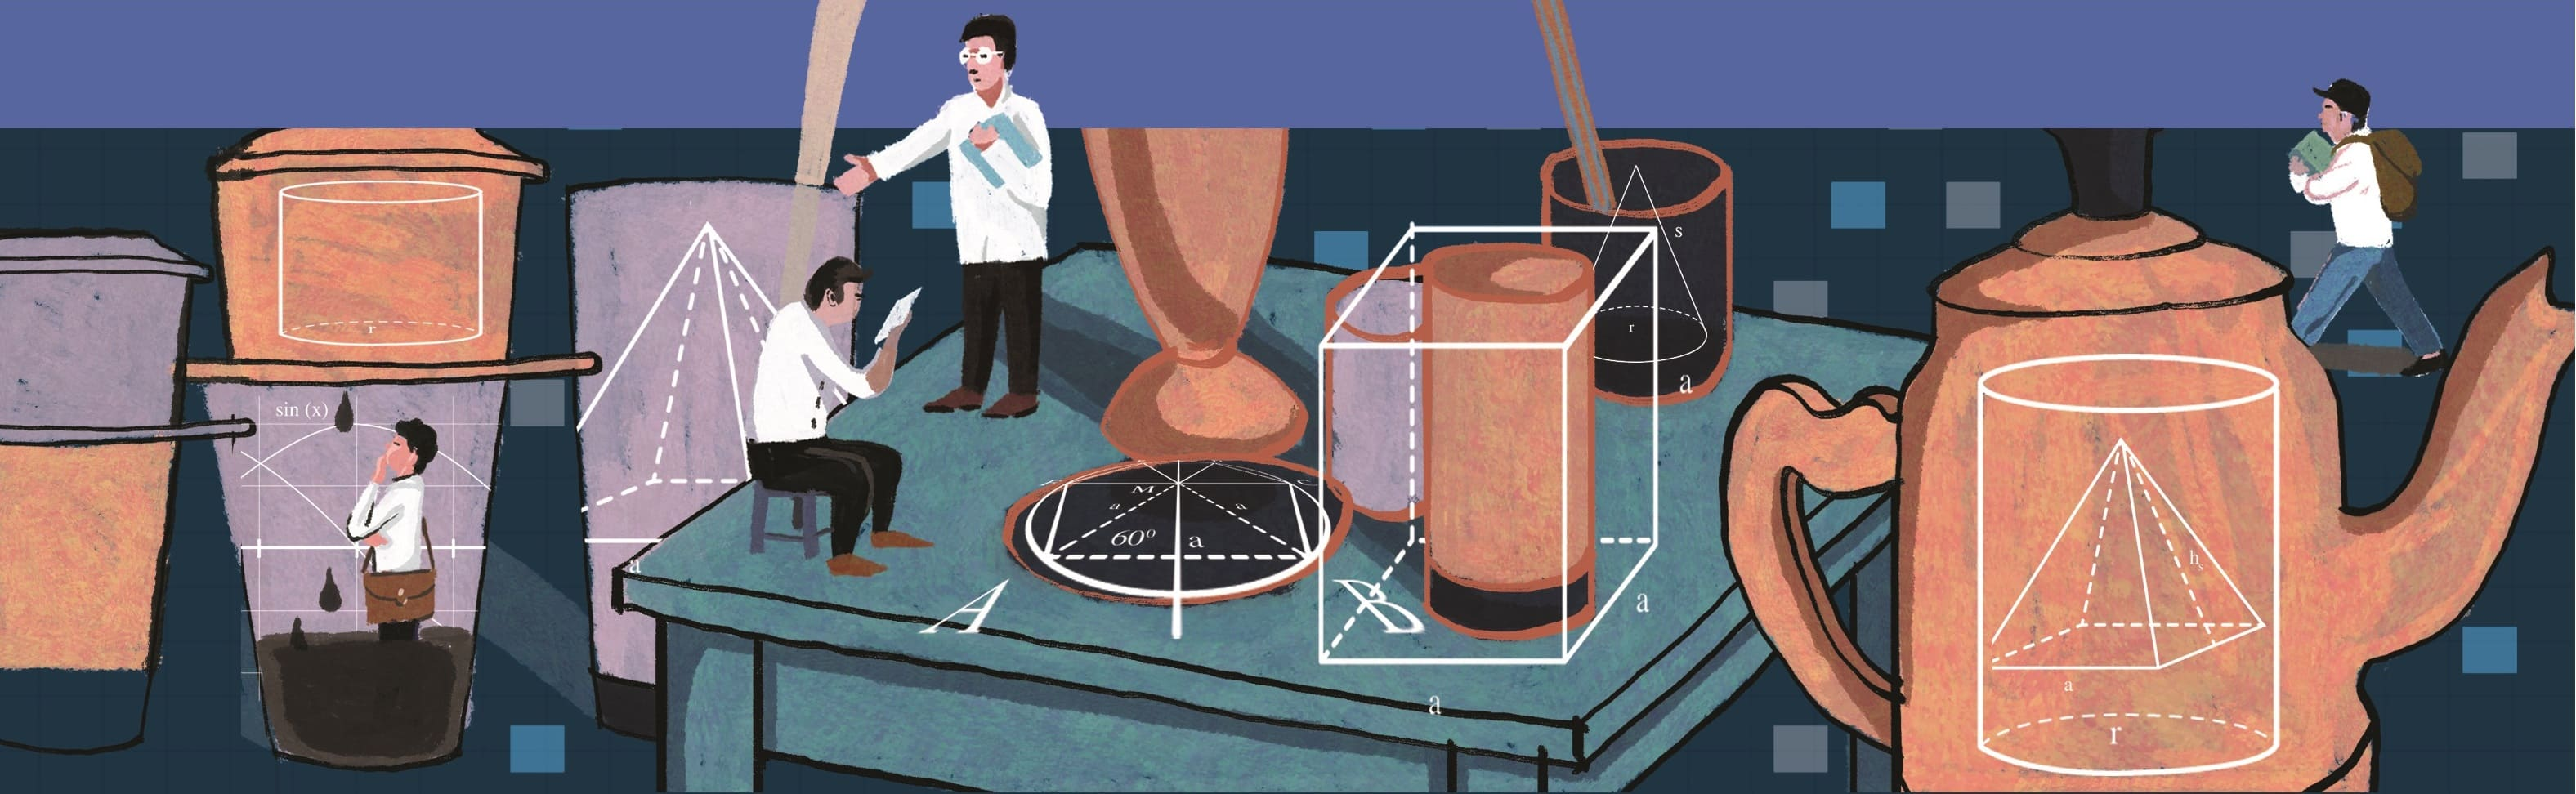
\includegraphics[width=19.3cm]{../bannerquantoan}}}
\AddToShipoutPicture*{\put(104,495){
\includegraphics[scale=1]{../tieude.pdf}}}
\centering
\endgroup

\vspace*{218pt}
\textit{\textbf{\color{quantoan}LTS.} Chuyên mục Danh ngôn Toán học giới thiệu với bạn đọc về lịch sử, ý nghĩa của những phát ngôn bởi các nhà toán học nổi tiếng. Ban biên tập Pi trân trọng mời bạn đọc đóng góp cho chuyên mục này.}

\vspace*{-5pt}
\begin{multicols}{2}
	Vào khoảng ba thế kỷ trước Công nguyên có một người Hy Lạp tên là Euclid từ xứ Alexandria. Họ gọi ông là như vậy, vì không ai biết họ của ông là gì. Ông lang thang ở thành Alexandria và trong thời gian rỗi, ông đã viết ra một bộ sách giáo khoa về hình học mà ông đặt tên là Cơ sở. Có lẽ ông đã được đào tạo sớm từ các học trò của Plato ở Athens, sau đó tiếp tục thành lập một trường học ở Alexandria vào năm $306$ trước Công nguyên. 
	\vskip 0.1cm
	Vào thời đó, có một nhà cai trị và tướng quân người Macedonia thuộc Hy lạp  là Ptolemy I Soter . Ông từng là vệ sỹ riêng của Alexander Đại đế, cũng đồng thời là một pharaoh của Ai Cập. Ptolemy I, giống như Alexander, rất quan tâm đến việc thúc đẩy nghiên cứu học thuật, và ông là người bảo trợ cho việc khai phá tri thức, sáng lập ra Đại Thư viện Alexandria. Ông ta tập hợp những ``người có học" xung quanh cung đình của mình.  Những người được biết đến là ``các bạn bè" này, bất kể là người đó là quý tộc hay thường dân, phục vụ Ptolemy với vai trò là các cố vấn chính của ông. Danh tiếng về bản tính nhân từ và phóng khoáng của tướng quân Ptolemy I đã gắn kết tầng lớp lính tráng trôi nổi nay đây mai đó, gồm cả những người Macedonia và những người Hy Lạp khác  tới phục vụ quanh ông. Chính Ptolemy đã viết cuốn Sử lược về các chiến dịch của Alexander, đã thất truyền. Đây từng được coi là một tác phẩm khách quan, nổi bật bởi tính trung thực và sự tỉnh táo trong nhận định. 
	\begin{figure}[H]
		\vspace*{-5pt}
		\centering
		\captionsetup{labelformat= empty, justification=centering}
		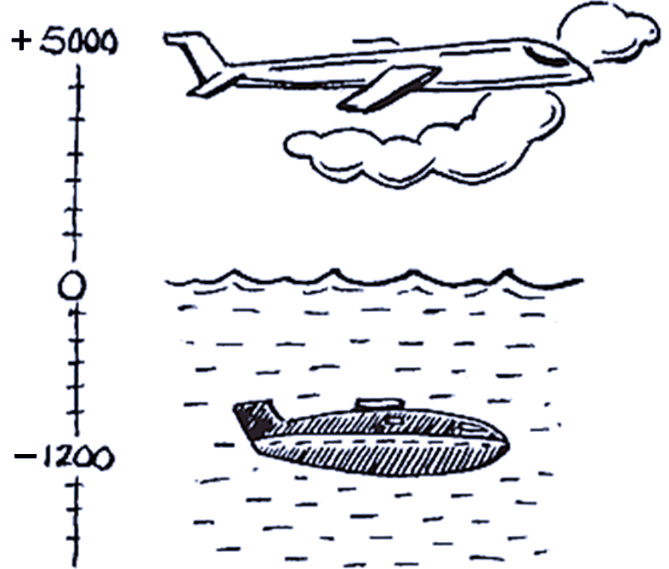
\includegraphics[width= 1\linewidth]{1}
		\caption{\small\textit{\color{quantoan}Hình $1$. Ptolemy I Soter ($366-282$ TCN), vị pharaoh Ai cập đồng thời là tướng quân người Macedonia thuộc Hy lạp.}}
		\vspace*{-12pt}
	\end{figure}
	Ptolemy I cũng  từng mời Triết gia nổi tiếng Strabo đến Alexandria làm gia sư cho con trai mình. Và khá đặc biệt, nhà toán học Euclid cũng là một trong những học giả được Prolemy bảo trợ. Tướng quân Ptolemy thấy tác phẩm tiêu biểu của Euclid, cuốn Cơ sở, quá khó để lĩnh hội, vì vậy ông ta  đã hỏi liệu có cách nào dễ dàng hơn để nắm vững được nó không. Và Euclide, theo ghi chép lại của Triết gia Proclus, đã có câu nói châm biếm nổi tiếng sau để trả lời Ptolemy ``Thưa Đức Ngài, không có con đường hoàng gia nào dẫn tới hình học".
	\begin{figure}[H]
		\vspace*{-5pt}
		\centering
		\captionsetup{labelformat= empty, justification=centering}
		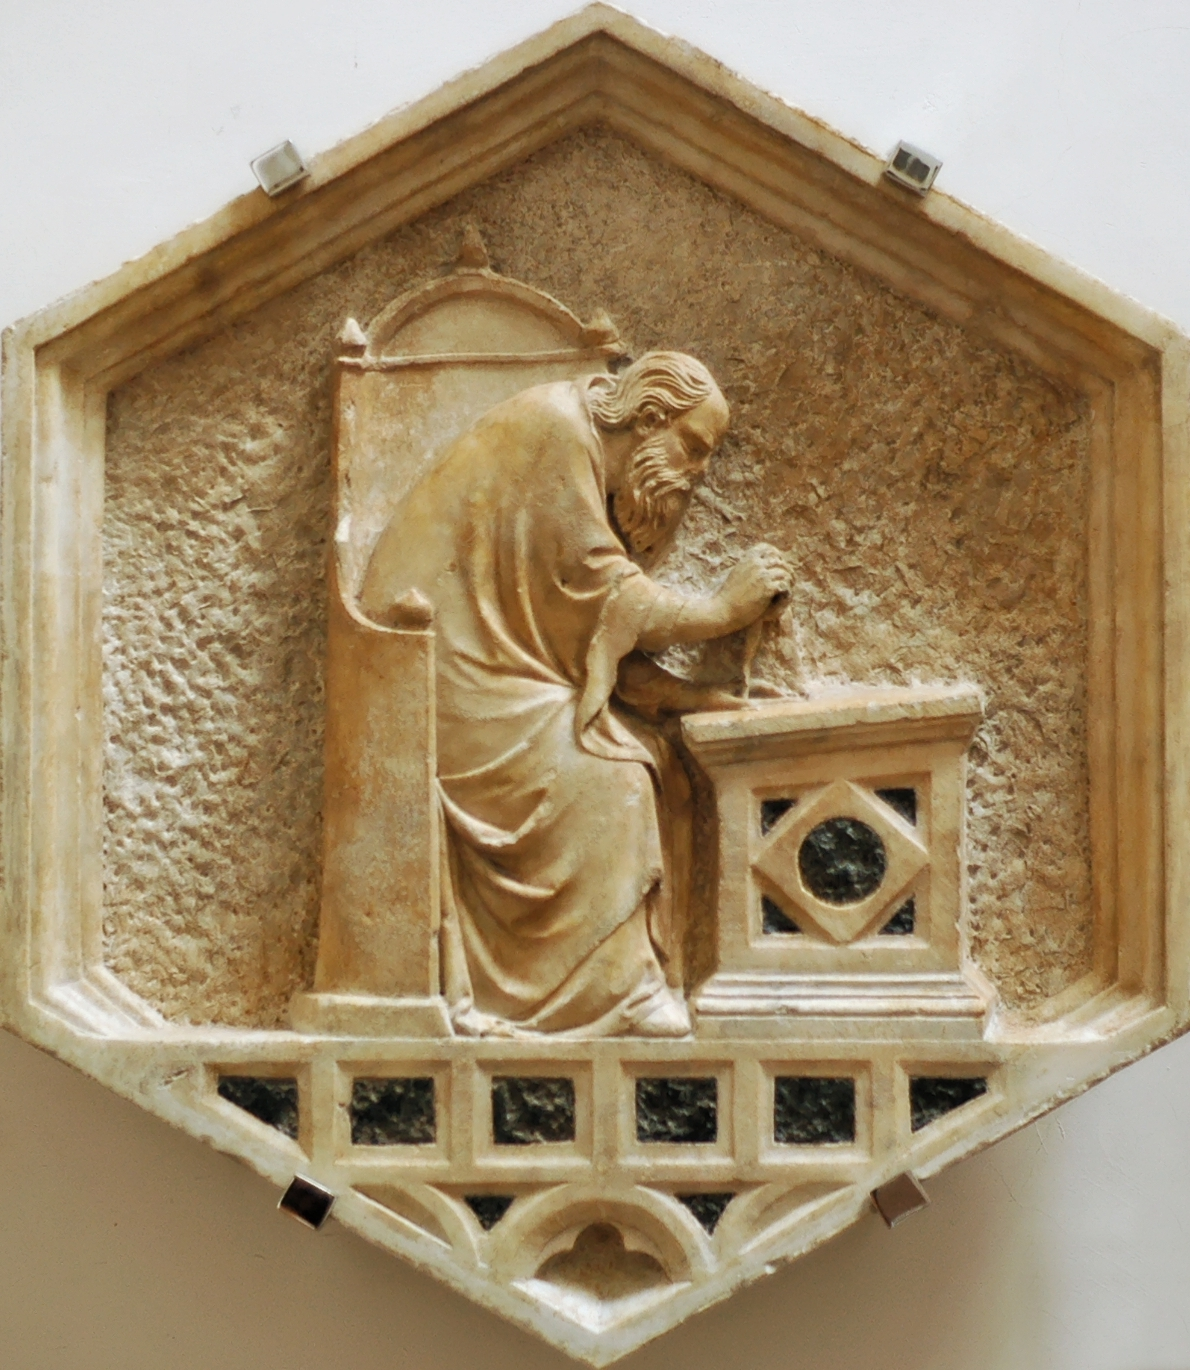
\includegraphics[width= 0.6\linewidth]{4}
		\caption{\small\textit{\color{quantoan}Hình $3$. Euclid, hay Kiến trúc. Tranh đá cẩm thạch, tầng hầm tháp chuông Florence, Ý.}}
		\vspace*{-10pt}
	\end{figure}
	Cụm từ ``Con đường Hoàng gia" thời đó chỉ  con đường đặc biệt được xây dựng xuyên qua Anatolia và Ba Tư bởi Darius Đại đế của Ba Tư (Darius I), cho phép liên lạc và chuyển quân nhanh chóng, nhưng Euclide đã sử dụng từ Hy lạp  ἀτραπός nghĩa là ``lối đi" (chứ không phải từ ὁδός ``con đường")  để truyền đạt ý nghĩa của ``đường tắt".
	\begin{figure}[H]
		\vspace*{-5pt}
		\centering
		\captionsetup{labelformat= empty, justification=centering}
		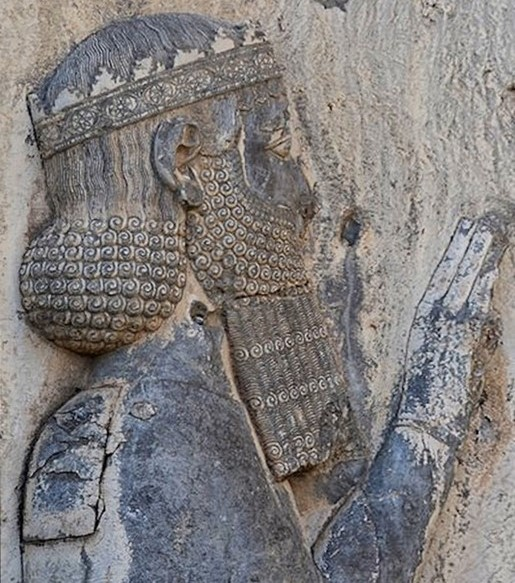
\includegraphics[width= 0.6\linewidth]{2}
		\caption{\small\textit{\color{quantoan}Hình $3$. Darius Đại đế của Ba Tư ($550-486$ TCN).}}
		\vspace*{-10pt}
	\end{figure}
	Tất nhiên, Eclide đã  nói bằng tiếng Hy Lạp với hy vọng Ptolemy sẽ hiểu ra rằng không có một điểm tín chỉ thưởng nào cho những ai chỉ đơn giản có mặt để điểm danh qua loa, khi muốn học môn hình học cho đến nơi đến chốn.
	\vskip 0.1cm
	Rất thú vị, ngày nay cụm từ ``con đường hoàng gia" đã vượt qua khuôn khổ của hình học và toán học, với ý nghĩa mới là ``con đường dẫn tới đích dễ dàng và nhanh nhất, không tốn công sức". Người ta có thể nói, ``đội bóng, sau khi đã loại tất cả các đối phương trong cùng nhóm, hiện đang trên con đường hoàng gia dẫn tới chức vô địch lần đầu tiên trong lịch sử thông qua đá loại trực tiếp", ``hãng phim nọ đang trên con đường hoàng gia đơn độc thống trị cả nền sản xuất điện ảnh và  tạo ra một thế độc quyền trong nền công nghiệp mà họ đang tích cực khai thác". Và tất nhiên, khi học tiếng Anh, các bạn cũng đều biết tới câu nói ``there is no royal road to learning". Học tiếng Anh, cũng như học hình học, đòi hỏi phải luyện tập kiên trì để đạt tới thành công trong việc diễn tả lưu loát những ý nghĩ riêng của bản thân mà không phải học thuộc lòng những cách nói mẫu, tuy đẹp nhưng khác lạ với cách diễn đạt của chính mình. 
	\begin{figure}[H]
		\vspace*{-5pt}
		\centering
		\captionsetup{labelformat= empty, justification=centering}
		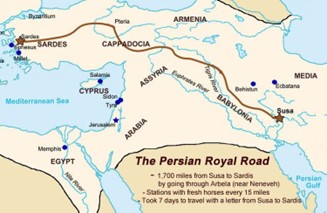
\includegraphics[width= 1\linewidth]{3}
		\caption{\small\textit{\color{quantoan}Hình $4$. Con đường Hoàng gia của Ba Tư.}}
		\vspace*{-10pt}
	\end{figure}
	Còn trong môn hình học, cần rất nhiều kiên trì để hiểu và ghi nhớ những điều phức tạp của môn học, bao gồm các tính chất khác nhau của các hình khác nhau có hai chiều và ba chiều. Chỉ khi đó chúng ta mới có thể học được cách dựng và phân tích các hình hình học.
\end{multicols}